
\medskip

Pour savoir si les feux de croisement de sa voiture sont réglés correctement, Pauline éclaire un mur vertical comme l'illustre le dessin suivant: 

\begin{center}
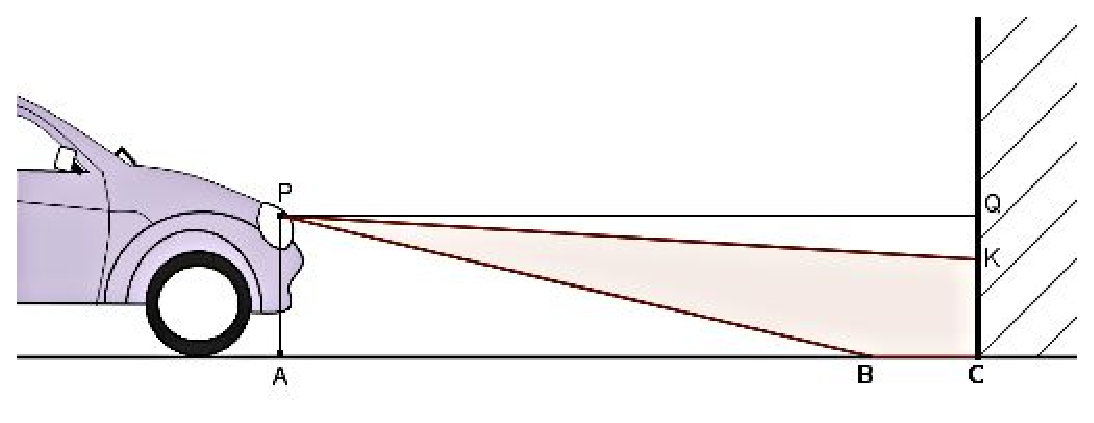
\includegraphics[width=10cm]{images-002.eps} 
\end{center}

%\begin{center}
%\psset{unit=1cm}
%\begin{pspicture}(10,5)
%\psline(0,0.5)(10,0.5)
%\psframe[linewidth=0pt,fillstyle=vlines](8,0.5)(10,2.5)
%\psline(2,2)(2,0.5)
%\psline(2,2)(8,2)
%\psline(2,2)(8,1.5)
%\psline(2,2)(7,0.5)
%\uput[d](7,0.5){B}
%\uput[d](8,0.5){C}
%\uput[r](8,1.5){K}
%\uput[r](8,2){O}
%\uput[u](2,2){P}
%\uput[d](2,0.5){A}
%\rput{-60}(1.8,1.8){\psellipse(0,0)(0.4,0.3)}
%\pspolygon[fillstyle=solid,fillcolor=cyan](2,2)(8,1.5)(8,0.5)(7,0.5)
%\rput(1,1.5){phare}
%\end{pspicture}
%\end{center}

Pauline réalise le schéma ci-dessous (qui n'est pas à l'échelle) et relève les mesures suivantes : 

PA = 0,65 m, AC = QP = 5 m et CK = 0,58 m. 

P désigne le phare, assimilé à un point. 

\begin{center}
\psset{xunit=0.4cm,yunit=1cm}
\begin{pspicture}(25,5)
%\psgrid
\psline(0,0.5)(25,0.5)
\psline(2,2)(2,0.5)
\psline(2,2)(8,2)
\psline(2,2)(24,0.5)
\psline(2,2)(7,0.5)
\uput[d](7,0.5){B}
\uput[d](8,0.5){C}
\uput[r](8,1.4){K}
\uput[r](8,2){Q}
\uput[u](2,2){P}
\uput[d](2,0.5){A}
\psframe(8,2)(7.6,1.8)
\psframe(8,0.5)(7.6,0.7)
\psline(8,2)(8,0.5)
\uput[d](24,0.5){S}
\end{pspicture}
\end{center}

Pour que l'éclairage d'une voiture soit conforme, les constructeurs déterminent l'inclinaison du faisceau. Cette inclinaison correspond au rapport $\dfrac{\text{QK}}{\text{QP}}$ . Elle est correcte si ce rapport est compris entre 0,01 et 0,015. 

\medskip 

\begin{enumerate}
\item Vérifier que les feux de croisement de Pauline sont réglés avec une inclinaison égale à $0,014$. 
\item Donner une mesure de l'angle $\widehat{\text{QPK}}$ correspondant à l'inclinaison. On arrondira au dixième de degré. 
\item Quelle est la distance AS d'éclairage de ses feux ? Arrondir le résultat au mètre près. 
\end{enumerate}

\vspace{0,5cm} 

